\documentclass[14pt]{beamer}

\usetheme[secheader]{Boadilla}

% Presento style file
\usepackage{tikz}
\usetikzlibrary{tikzmark,fit,shapes.geometric}

% Information
\title{Courbes planes paramétrées}
\subtitle{Partie 2}
\author{Y. Carissan}
%\institute{www.ratulsaha.com}
\date{2020}

\AtBeginSection[]{\begin{frame}{Plan}\tableofcontents[currentsection,hideothersubsections]\end{frame}}

\begin{document}

% Title page
\begin{frame}{}
\maketitle
\end{frame}

\begin{frame}{Plan}
        \tableofcontents[hideallsubsections]
\end{frame}

\section{Courbes planes en paramétrage polaire}
\subsection{Coordonnées polaires}
\begin{frame}
        \begin{alertblock}{Définition~:}
                Soit un point du plan $M$ tel que $M\ne O$.\\
                Soit $\vec{u}$ un vecteur directeur unitaire de $\vec{OM}$.\\
                On appelle coordonnées polaires de $M$ le couple $(\theta;r)$
                tels que~:
                \begin{align*}
                        \left\{\begin{array}{l}
                                \theta = \widehat{(\vec{i}, \vec{u})}\\
                                \vec{OM} = r\vec{u}
                        \end{array}\right.
                \end{align*}
        \end{alertblock}
\end{frame}
\begin{frame}
        \begin{block}{Méthode}
                On place successivement~:
                \begin{enumerate}
                                \item<1-> $\theta$
                                \item<2-> $\vec{u}$ grâce à la formule $\theta = \widehat{(\vec{i}, \vec{u})}$
                                \item<3-> $M$ grâce à la formule $\vec{OM} = r\vec{u}$
                \end{enumerate}
                \begin{center}
                        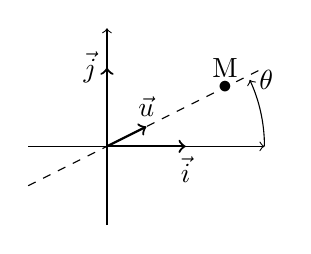
\begin{tikzpicture}
                                \draw[->] (-1,0) -- (2,0);
                                \draw[->] (0,-1.0) -- (0,1.5);
                                \onslide<1>{\draw[->,thick] (0,0) -- (1,0) node [below] {$\vec{i}$};
                                \draw[->,thick] (0,0) -- (0,1) node [left] {$\vec{j}$};}
                                \draw[dashed] (-1,-0.5) -- (2,1);
                                \onslide<1>{\draw[->] (2,0) arc(0:25:2) node [right] {$\theta$};}
                                \onslide<2>{\draw[->,thick] (0,0) -- (0.5,0.25) node [above] {$\vec{u}$};}
                                \onslide<3>{\draw (1.5,0.75) node {$\bullet$} node [above] {M};}
                        \end{tikzpicture}
                \end{center}
        \end{block}
\end{frame}
\end{document}
